% Augmented Reality

\chapter{Augmented Reality} % Main chapter title

\label{AugmentedReality}

%----------------------------------------------------------------------------------------

This chapter covers the AR portion of the project. The AR subsystem takes the positions from the position calculation subsystem and renders them on the screen of a cellphone using OpenGL. If they cannot be directly rendered, an arrow is drawn on the edge of the screen to show which way the object is from the user. An example of this can be found in Figure~\ref{dfis} (DO THIS FIGURE).

The code for the AR subsystem can be found at (PROVIDE LINK HERE).

This chapter covers the following topics:
\begin{enumerate}
	\item A brief overview of the math used later in this section, including homogenous coordinates and transformation matrices.
	\item A description of OpenGL and the basics of how it is used. 
	\item How objects and text can accurately be drawn on the screen overlaid on a camera image.
	\item How the coordinate system of the position calculation system can be transformed into real world coordinates through the cell phone's sensors.
	\item Examples of the accuracy of the subsystem.
\end{enumerate}

\section{3D Math Overview}
This section covers the basics of using matrices to render 3D scenes. A full treatment of the subject is beyond the scope of this report.. The reader is assumed to be familiar with some linear algebra, including the multiplication of matrices. 

\subsection{Transformation Matrices}
\begin{figure}
	\centering
	\begin{minipage}{.33\textwidth}
		\centering
		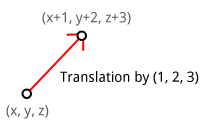
\includegraphics[width=\linewidth]{Figures/Translation.png}
	\end{minipage}
	\begin{minipage}{.33\textwidth}
		\centering
		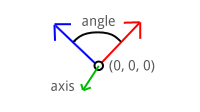
\includegraphics[width=\linewidth]{Figures/Rotation.png}
	\end{minipage}
	\begin{minipage}{.33\textwidth}
		\centering
		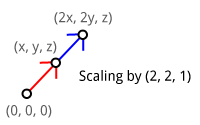
\includegraphics[width=\linewidth]{Figures/Scaling.png}
	\end{minipage}
	\decoRule
	\caption{Translation, rotation, and scaling of vectors are all possible with matrices \cite{OpenGLMatrices}.}
	\label{fig:Transformations}
\end{figure}

\textbf{Transformation matrices} are matrices which can describe transformations in space such as translation, rotation, and scaling. They are regularly used in computer graphics. 

Figure~\ref{fig:Transformations} shows some of the transformations that can be applied to vertices with matrices.

Transform matrices can be composed with multiplication. For example, one could describe the translation of a point with a translation matrix, then multiply the matrix by a rotation matrix to create a new matrix which, when multiplied by a vector, cause that vector to be rotated and then translated.

Order matters when composing transformation matrices. The matrix $\mathbf{T} \mathbf{R}$ is not the same as $\mathbf{R} \mathbf{T}$.

Normally, the transformation of a vector $v$ to a new vector $v'$ with a transformation matrix $\mathbf{M}$ is written as:

\[ v' = \mathbf{M} v \]

Or, with two transformation matrices $\mathbf{M_1}$ and $\mathbf{M_2}$ composed:

\[ v' = \mathbf{M_2} \mathbf{M_1} v \]

When written like this, the transformation matrix $\mathbf{M_1}$ can be viewed as applying to the vector first, and then the new transformed will be further transformed by $\mathbf{M_2}$.

In this report, points and vectors will be used interchangeably. When a matrix is said to multiply a point $p = (x, y, z)$, it should be considered as multiplying a vector $v = \begin{bmatrix}x & y & z\end{bmatrix}^T $. 

The definitions of matrices which scale, translate, and rotate are beyond the scope of this report. OpenGL provides utility functions to create such matrices, so the exact definitions are unnecessary.

\subsection{Homogenous Coordinates}
For a given 3$\times$3 matrix $M$ and an arbitrary point in 3D space $p = (x, y, z)$, there is no $\mathbf{M}$ such that will multiplying it by any $p$ will cause $p$ to be translated by a specified number of units. There is, however, a way to do it with a homogenous point and a 4x4 matrix. This is one of the reasons homogenous coordinates are used in OpenGL.

\textbf{Homogenous coordinates} are coordinates in space which contain an extra element $w$ which acts as a scaling factor on the three elements. A 3D homogenous coordinate $p_h$ could be written as:

\[ p_h = (x_h, y_h, z_h, w) \]

This relates to a regular point in 3D space:

\[ (x, y, z) = (\frac{x_h}{w}, \frac{y_h}{w}, \frac{z_h}{w}) \] 

For example, the homogenous point $(1, 1, 1, 1)$ maps to the regular 3D point $(1, 1, 1)$. The homogenous point $(2, 2, 2, 2)$ does as well.

A translation matrix $T$ that moves a point $p$  by $(T_x, T_y, T_z)$ units, is:

\[
\mathbf{T} = \begin{bmatrix}
1 & 0 & 0 & T_x \\
0 & 1 & 0 & T_y \\
0 & 0 & 1 & T_z \\
0 & 0 & 0 & 1
\end{bmatrix}
\]

To prove this, we'll multiply out a homogenous point $p_h = (x_h, y_h, z_h, w)$ by $\mathbf{T}$ and show that, when converted to a regular 3D point, it equals $(\frac{x}{w} + T_x, \frac{y}{w} + T_y, \frac{z}{w} + T_z)$.

\[ p_{h}\prime = \mathbf{T} p_h \]

\[
  p_{h}\prime = \begin{bmatrix}
1 & 0 & 0 & T_x \\
0 & 1 & 0 & T_y \\
0 & 0 & 1 & T_z \\
0 & 0 & 0 & 1
\end{bmatrix} 
\begin{bmatrix}
x_h \\ y_h \\ z_h \\ w 
\end{bmatrix}
\]

\[
 p_{h}\prime = \begin{bmatrix}
 x_h + w T_x \\
 y_h + w T_y \\
 z_h + w T_z \\
 w
 \end{bmatrix}
 \]
 
 Now, if we convert $p_{h}\prime$ to a regular 3D point $p$, we get:
 
 \[ p = (\frac{x_h}{w} + \frac{w T_x}{w},  \frac{y_h}{w} + \frac{w T_y}{w}, \frac{z_h}{w} + \frac{w T_z}{w}) \]
 \[ p = (x/w + T_x, y/w + T_y, z/w + T_z) \]
 
 which is the translation of $p$ by $(T_x, T_y, T_z)$ units.
 
\section{OpenGL}
\textbf{OpenGL} is an API used to render 2D and 3D graphics. In the project, OpenGL was used to render position markers in 3D space overtop what the cell phone's camera sees.

OpenGL works by taking in collections of points making up a 3D model of an object and then applying various matrix transforms to the points, translating and rotating them. Afterwards, it projects them onto a 2D plane and renders them. A full treatment of how OpenGL works is beyond the scope of this report.

The three main matrices that OpenGL uses to render a 3D scene are called the \textbf{projection matrix}, \textbf{view matrix}, and \textbf{model matrix}. This project uses several novel techniques which use and manipulate the matrices that OpenGL uses to render a 3D scene. This report will only cover them briefly, though other resources explore them more fully \cite{CodingLabs}.

\section{The Model Matrix}
\begin{figure}
	\centering
	\tikzstyle{vertex}=[circle, draw]
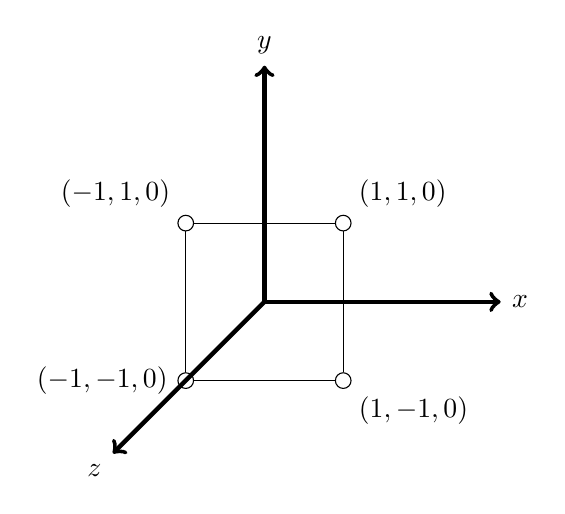
\begin{tikzpicture}[transform shape]
\draw[->,ultra thick] (0,0, 0)--(3,0, 0) node[right]{$x$};
\draw[->,ultra thick] (0,0, 0)--(0,3, 0) node[above]{$y$};
\draw[->,ultra thick] (0,0, 0)--(0,0, 5) node[below left]{$z$};

\node[vertex,inner sep=2pt,minimum size=1pt,label=left:{$(-1, -1, 0)$}](v1) at (-1, -1, 0) {};
\node[vertex,inner sep=2pt,minimum size=1pt,label=below right:{$(1, -1, 0)$}](v2) at (1, -1, 0) {};
\node[vertex,inner sep=2pt,minimum size=1pt,label=above right:{$(1, 1, 0)$}](v3) at (1, 1, 0) {};
\node[vertex,inner sep=2pt,minimum size=1pt,label=above left:{$(-1, 1, 0)$}](v4) at (-1,1, 0) {};

\begin{scope}[every path/.style={-}, every node/.style={inner sep=0pt}]
       \draw (v1) -- node [anchor=south east] {} (v2);
       \draw (v2) -- node [anchor=south west] {} (v3);
       \draw (v3) -- node [anchor=north] {} (v4);
       \draw (v4) -- node [anchor=north] {} (v1);
\end{scope} 
\end{tikzpicture}
	\decoRule
	\caption{An example 3D model of a square in model coordinates.}
	\label{fig:ModelExample}
\end{figure}
\begin{figure}
	\centering
	\tikzstyle{vertex}=[circle, draw]
\begin{tikzpicture}[transform shape={scale=0.4}]
\draw[->,ultra thick] (0,0, 0)--(5,0, 0) node[right]{$x$};
\draw[->,ultra thick] (0,0, 0)--(0,5, 0) node[above]{$y$};
\draw[->,ultra thick] (0,0, 0)--(0,0, 5) node[below left]{$z$};

\node[vertex,inner sep=2pt,minimum size=1pt,label=below:{$(-6, -1, 0)$}](v1) at (-6, -1, 0) {};
\node[vertex,inner sep=2pt,minimum size=1pt,label=below right:{$(-4, -1, 0)$}](v2) at (-4, -1, 0) {};
\node[vertex,inner sep=2pt,minimum size=1pt,label=above right:{$(-4, 1, 0)$}](v3) at (-4, 1, 0) {};
\node[vertex,inner sep=2pt,minimum size=1pt,label=above:{$(-6, 1, 0)$}](v4) at (-6,1, 0) {};

\node[vertex,inner sep=2pt,minimum size=1pt,label=left:{$(4, -1, 0)$}](v5) at (4, -1, 0) {};
\node[vertex,inner sep=2pt,minimum size=1pt,label=below right:{$(6, -1, 0)$}](v6) at (6, -1, 0) {};
\node[vertex,inner sep=2pt,minimum size=1pt,label=above right:{$(6, 1, 0)$}](v7) at (6, 1, 0) {};
\node[vertex,inner sep=2pt,minimum size=1pt,label=above left:{$(4, 1, 0)$}](v8) at (4,1, 0) {};

\begin{scope}[every path/.style={-}, every node/.style={inner sep=0pt}]
       \draw (v1) -- node [anchor=south east] {} (v2);
       \draw (v2) -- node [anchor=south west] {} (v3);
       \draw (v3) -- node [anchor=north] {} (v4);
       \draw (v4) -- node [anchor=north] {} (v1);
       
       \draw (v5) -- node [anchor=south east] {} (v6);
       \draw (v6) -- node [anchor=south west] {} (v7);
       \draw (v7) -- node [anchor=north] {} (v8);
       \draw (v8) -- node [anchor=north] {} (v5);
\end{scope} 
\end{tikzpicture}
	\decoRule
	\caption{A 3D scene with two squares, the centers of which are placed at $(5, 0, 0)$ and $(-5, 0, 0)$ in world coordinates by transforming the vertices of Figure~\ref{fig:ModelExample} with two model matrices.}
	\label{fig:ModelMatrixExample}
\end{figure}

The model matrix exists to take \textbf{model space}, in which the coordinates of a 3D model are relative to the center of the model, and transform it into \textbf{world space}, in which coordinates are relative to the center of the ``world''. Most of the code in this project considers the locations of objects in world space. For example, the position subsystem might say that a tag is at $(5, 5, 1)$. This coordinate is considered to be in world space, though it should be noted that this is not the same as \emph{real} world coordinates - a further transform is required to match up the positions given by the position calculation subsystem with the real world as shown by a camera.

Figure~\ref{fig:ModelExample} shows an example of a square in model space. The square's 3D model has its vertices placed at $(-1, -1, 0)$, $(1, -1, 0)$, $(1, 1, 0)$, and $(-1, 1, 0)$. An example of creating a 3D scene with two squares at $(5, 0, 0)$ and $(-5, 0, 0)$ in world coordinates can be seen in Figure~\ref{fig:ModelMatrixExample}. A model matrix is created for each of the squares. The first model matrix encodes a translation $(-5, 0, 0)$ units and the second model matrix encodes a translation of $(5, 0, 0)$ units. To get the vertices of the first square in world coordinates, the first model matrix is applied to the square's vertices. The same is done for the second square and model matrix. 

That is, for the model matrix $\mathbf{M}$ and each vertex $v$ of the square, the vertex $v$ is transformed into world coordinates vertex $v'$ by the formula:

\[v' = \mathbf{M}v \]

\section{The View Matrix}
\begin{figure}
	\centering
	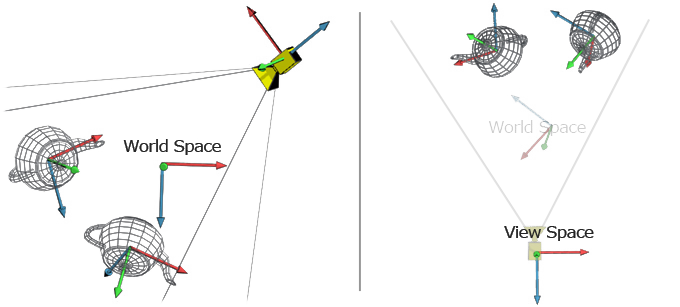
\includegraphics[width=\linewidth]{Figures/WorldToView.png}
	\decoRule
	\caption{A figure showing an object in world coordinates and an object in camera coordinates \cite{CodingLabs}.}
	\label{fig:WorldToView}
\end{figure}

In a 3D scene, a position is declared from which the scene is viewed. The view matrix exists to transform world coordinates to \textbf{view space}, in which coordinates are relative to the position from which the scene is viewed. It as if an imaginary camera has been placed in the scene. Figure~\ref{fig:WorldToView} shows an example of this.

The view matrix is typically just a simple translation of all the vertices (if a camera is placed at $(5, 5, 5)$, then all the vertices will be translated by $(-5, -5, -5)$), and then a rotation based in which direction the camera is looking at. 

For the rest of this project, the imaginary camera is assumed to be located at (0, 0, 0), making the view matrix a simple rotation matrix. The positions of markers and objects are calculated relative to the position of the tag connected to the cellphone.

\section{The Projection Matrix}

\begin{figure}
	\centering
	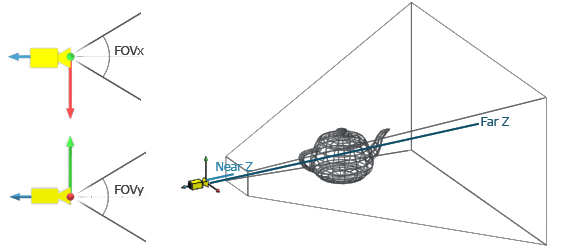
\includegraphics[width=\linewidth]{Figures/ProjectionMatrix.png}
	\decoRule
	\caption{The transformation from view space to projection space \cite{CodingLabs}.}
	\label{fig:ProjectionMatrix}
\end{figure}

\begin{figure}
	\centering
	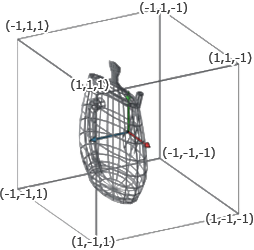
\includegraphics{Figures/ProjectionMatrix2.png}
	\decoRule
	\caption{A teapot in projection space \cite{CodingLabs}.}
	\label{fig:ProjectionMatrix2}
\end{figure}

In one of the last steps in rendering a 3D scene in OpenGL, the scene must be projected onto a plane so it can be displayed on a monitor. The projection matrix is involved in this process. View space is transformed into \textbf{projection space}, in which coordinates are transformed into \textbf{normalized device coordinates} (NDCs). Vertices which fall within the field of view will be contained within a cube with corners $(-1, -1, -1)$ and $(1, 1, 1)$ and are drawn. Vertices outside this box are culled. 

There are different types of projection matrices. For the purposes of this report, only the \textbf{perspective projection matrix} is considered. This projection takes into account that objects which are further away from the camera should appear smaller, which matches how a camera captures images. Figure~\ref{fig:ProjectionMatrix} and Figure~\ref{fig:ProjectionMatrix2} show the transform from view space to projection space via a perspective projection matrix.

To render the image in 2D, the NDCs are converted to the coordinates of pixels as determined by the size of the surface being rendered to. The $z$ coordinates handle depth, which allows OpenGL to determine whether a shape is on top of another during the rendering process.

\section{Camera Perspective and OpenGL Perspective}
\begin{figure}
	\centering
	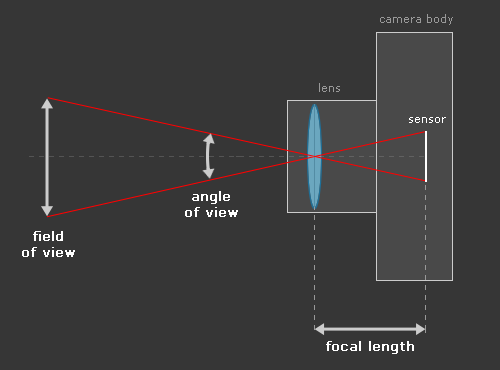
\includegraphics[width=\linewidth]{Figures/CameraLens.png}
	\decoRule
	\caption{A diagram depicting the field of view of a camera \cite{MartyBugs}.}
	\label{fig:CameraLens}
\end{figure}
In order to accurately display the locations of the devices, it is important that the 3D scene rendered by OpenGL match up with the real world as shown by the cellphone's camera. Figure~\ref{fig:CameraLens} shows how a camera can only see see a limited part of the world, as dictated by its field of view.

As previously shown in Figure~\ref{fig:ProjectionMatrix}, the projection matrix has a field of view which can be changed. The field of view for the OpenGL perspective matrix needs to be set on a per-cellphone basis to match that of the cellphone's camera for the project to display locations accurately.

The process of creating a projection matrix that properly matches the phone's camera is complex \cite{CalibratedCamera} and due to time constraints they were not able to be implemented in the project.

\section{Cellphone Rotation}
\begin{figure}
	\centering
	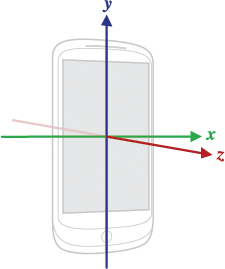
\includegraphics[width=6cm]{Figures/AxisDevice.png}
	\decoRule
	\caption{The coordinate system used by the Android Sensor API \cite{AndroidSensorDocsOverview} and by AR subsystem, assuming the phone's top points towards geomagnetic North and the screen points toward the sky. For the purposes of rotation, X points approximately East, Y to geomagnetic North, and Z towards the sky \cite{AndroidSensorDocs}.}
	\label{fig:RotationCoordinateSystem}
\end{figure}

In order to display the positions of markers on the screen correctly, the direction the camera is facing must be known. The cellphone can determine this by requesting the phone's rotation from Android's Sensor API. Android does not specify \emph{how} the rotation of the phone is determined, but in practice uses a subset of the magnetometer, accelerometer, and gyroscope (if the phone contains these sensors; Android does not force phone manufacturers to include any of these sensors). 

For example, if the phone has a magnetometer and an accelerometer, by determining the direction of magnetic north and the direction of the force of the gravity on the phone, the direction of the phone's rotation can be determined \cite{AndroidSensorDocs}.

The cellphone has its own coordinate system which must be taken into account. To deal with the coordinate system differences, the Android Sensor API includes a method to remap the coordinate system of the rotation it reports. The coordinate system used by the project for its real world coordinates was chosen to match the coordinate system of the Android Sensor API, which can be seen in Figure~\ref{fig:RotationCoordinateSystem}.

The rotation value returned by the Android OS was found to be quite accurate in tests so long as the device was not in motion. If the device was in freefall or moving, it became more difficult for the Android OS to determine the direction of gravity, which in turn made the calculated rotation values inaccurate.

The Android Sensor API can directly return a rotation matrix. However, the way it is stored in memory is not quite the same as how OpenGL stores matrices, so the matrix must be transposed before being used in OpenGL.

The rotation matrix returned is used in the project to create the view matrix by taking a ``lookAt'' vector equal to $(0, 0, -1)$ (which represents that the camera, when at `rest' on a table looks down the z axis) and ``up'' vector equal to $(0, 1, 0)$ (arbitrarily stating that the `up' direction of the cellphone screen points north) and rotating each by the rotation matrix returned by the phone. The new vectors produced are then used in the OpenGL utility function \code{setLookAtM} which creates a view matrix based on an up vector and the point at which the camera should be looking at.

The rotation matrix could have been used directly as the view matrix without going through these steps. However, it was found convenient to have the lookAt and up vectors rotated and available for use. 

If we ignore the transformation required to correct for the arbitrary coordinate system of the position calculation subsystem, the view matrix, $\mathbf{V}$, every frame is to set it equal to the rotation matrix the Android OS last returned, $\mathbf{R_{cur}}$:

\[
	\mathbf{V} = \mathbf{R_{cur}}
\]

\section{Calibration}
\label{Calibration}
As noted in Section~\ref{FrameOfReference}, the positions calculated by the position calculation subsystem have an arbitrary coordinate system where the XY plane is formed by the positions of the three anchors with the lowest ID and the Z axis is determined by the fourth anchor. In order to display positions obtained from this subsystem accurately on top of the images captured by the cellphone's camera, there is a necessary calibration step on system startup to create a transformation matrix which can convert coordinates into the cell phone's coordinate system. The user determines the transformation needed to convert to the coordinate system used by the cellphone by rotating and positioning the phone until it displays the position of a device correctly, at which point the system knows the transformation needed.

The steps a user follows to calibrate the system are:
\begin{enumerate}
	\item The user taps the phone's screen to enter calibration mode.
	\item The system creates a new view matrix every frame which will cause the screen to display the position of an arbitrary device in the network in the middle of the screen. The rotation of the phone is not taken into account for this view matrix.
	\item The user then points the phone directly at the tag being displayed and rotates the phone until the position of a second tag matches its location on the screen.
	\item The user then taps the screen to end calibration mode. The system stores the view matrix at this time, $\mathbf{V}_{end}$, as well as the raw rotation matrix at the time, $\mathbf{R}_{end}$.
	\item If the locations of other tags are incorrect due the z-axis being flipped (the z axis of the position calculation subsystem flips based on the elevation of the anchor with the highest ID), the user taps the phone's screen twice to correct it. The system stores this in a boolean and, when calculating the positions of other devices relative to the user's location, knows whether to flip the z component.
\end{enumerate}

(TODO INSERT PICTURE HERE)

Each frame, to correctly position the objects, the calibration matrix should be changed only by the rotation of the device from its rotation at the end of the calibration. Before, each frame the view matrix was set equal to the current raw rotation matrix, $\mathbf{R}_{cur}$. Now, the view matrix must multiplied by a matrix to correct for the coordinate transform. Intuitively, this calibration matrix should reverse the effects of the rotation at the end of the calibration mode and multiply by the view matrix at the time. A rotation can be reversed by inverting the matrix. Thus, the new calibrated view matrix used every frame, $\mathbf{V}_{cal}$, is:

\[ 
	\mathbf{V}_{cal} = \mathbf{V}_{end} \mathbf{R}^{-1}_{end} \mathbf{R}_{cur}
\]

\section{Billboarding}
\begin{figure}
	\centering
	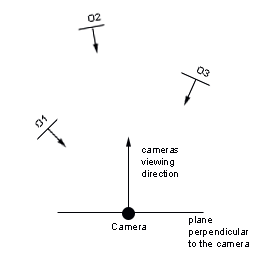
\includegraphics[width=8cm]{Figures/Billboarding.png}
	\decoRule
	\caption{Billboarding used to make objects O1, O2, and O3 face the camera \cite{Lighthouse3D}.}
	\label{fig:Billboarding}
\end{figure}
So far, this chapter has discussed how a collection of vertices can be transformed, and more specifically how the positions of other devices can be correctly placed. This would be sufficient if the system had to render a cube at the position of the object in question. Aesthetically, rendering a cube would leave a lot to be desired. This section covers a method to draw a 2D image at a 3D location.

\textbf{Billboarding} is a technique to make an object face the screen no matter where it is situated. It is used, for example, in some 3D games to render trees as 2D images to lower the number of vertices that need to be processed in a scene. Figure~\ref{fig:Billboarding} shows the end result of using billboarding for 2D objects.

There are many ways to do billboarding, depending on whether you want to only have the object rotate on a specific axis \cite{Lighthouse3D}. For this project, it was determined that the best way to represent an object's position on the screen was to have a rotating circular 2D image as a marker. The exact graphic used was chosen for aesthetic reasons.

To have this 2D image always face the screen, it must be able to rotate on all three axes. The technique to accomplish this rotation is to multiply the model matrix before it is translated by the inverse of the portion of the view matrix corresponding to rotation. That is, given a model matrix $\textbf{M}$, making it rotate to always face the camera is accomplished by creating a new billboarding model matrix $\textbf{M}_b$:

\[ \textbf{M}_b = \textbf{M} \textbf{V}^{-1} \]

Intuitively, when a model's vertices are multiplied by the view matrix, they are rotated about depending on the angle the camera is facing. If we reverse this rotation effect but not the translation part, the model will always face the camera.

As the camera is always situated at $(0, 0, 0)$ in this project, multiplying the model matrix of the textured square by the inverted view matrix will produce a billboarding effect. If we first rotate the square about the Z-axis (assuming the square's vertices are on the XY plane), it will produce the rotating effect on the final image.

\section{Marking the Positions of Objects Off-Screen}

\begin{figure}
	\centering
	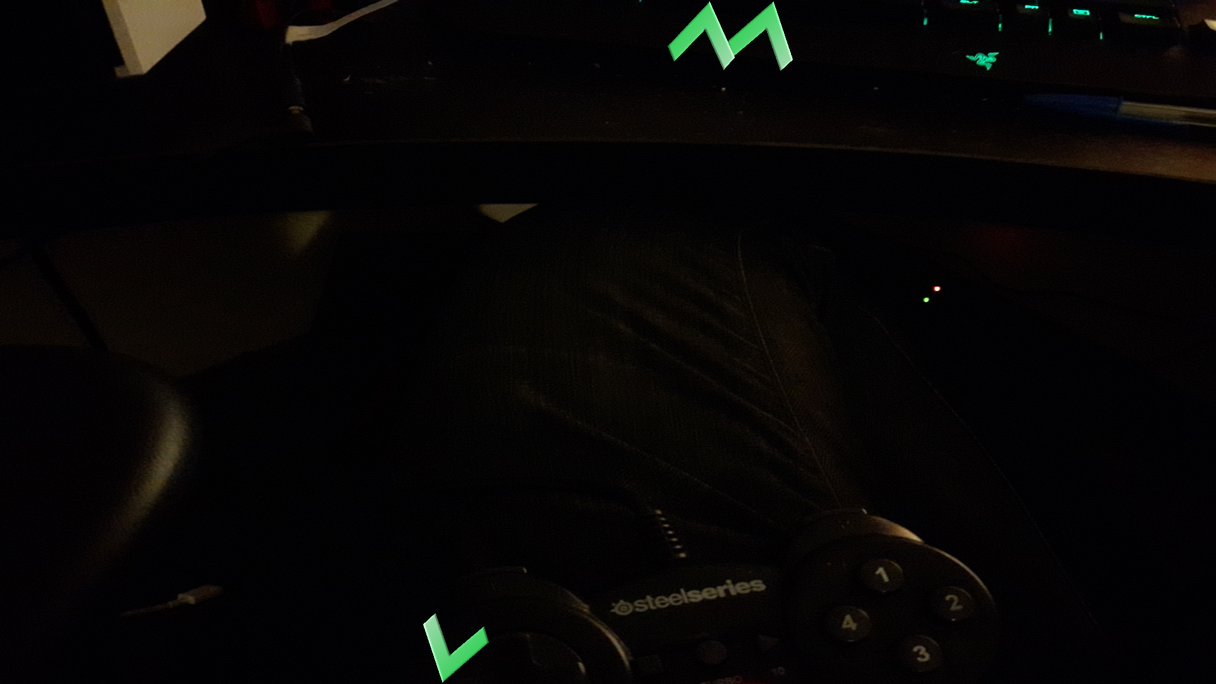
\includegraphics[width=8cm]{Figures/OffscreenPositions1.png}
	\decoRule
	\caption{Offscreen tag positions are shown with a green arrow}
	\label{fig:Billboarding}
\end{figure}

begin{figure}
	\centering
	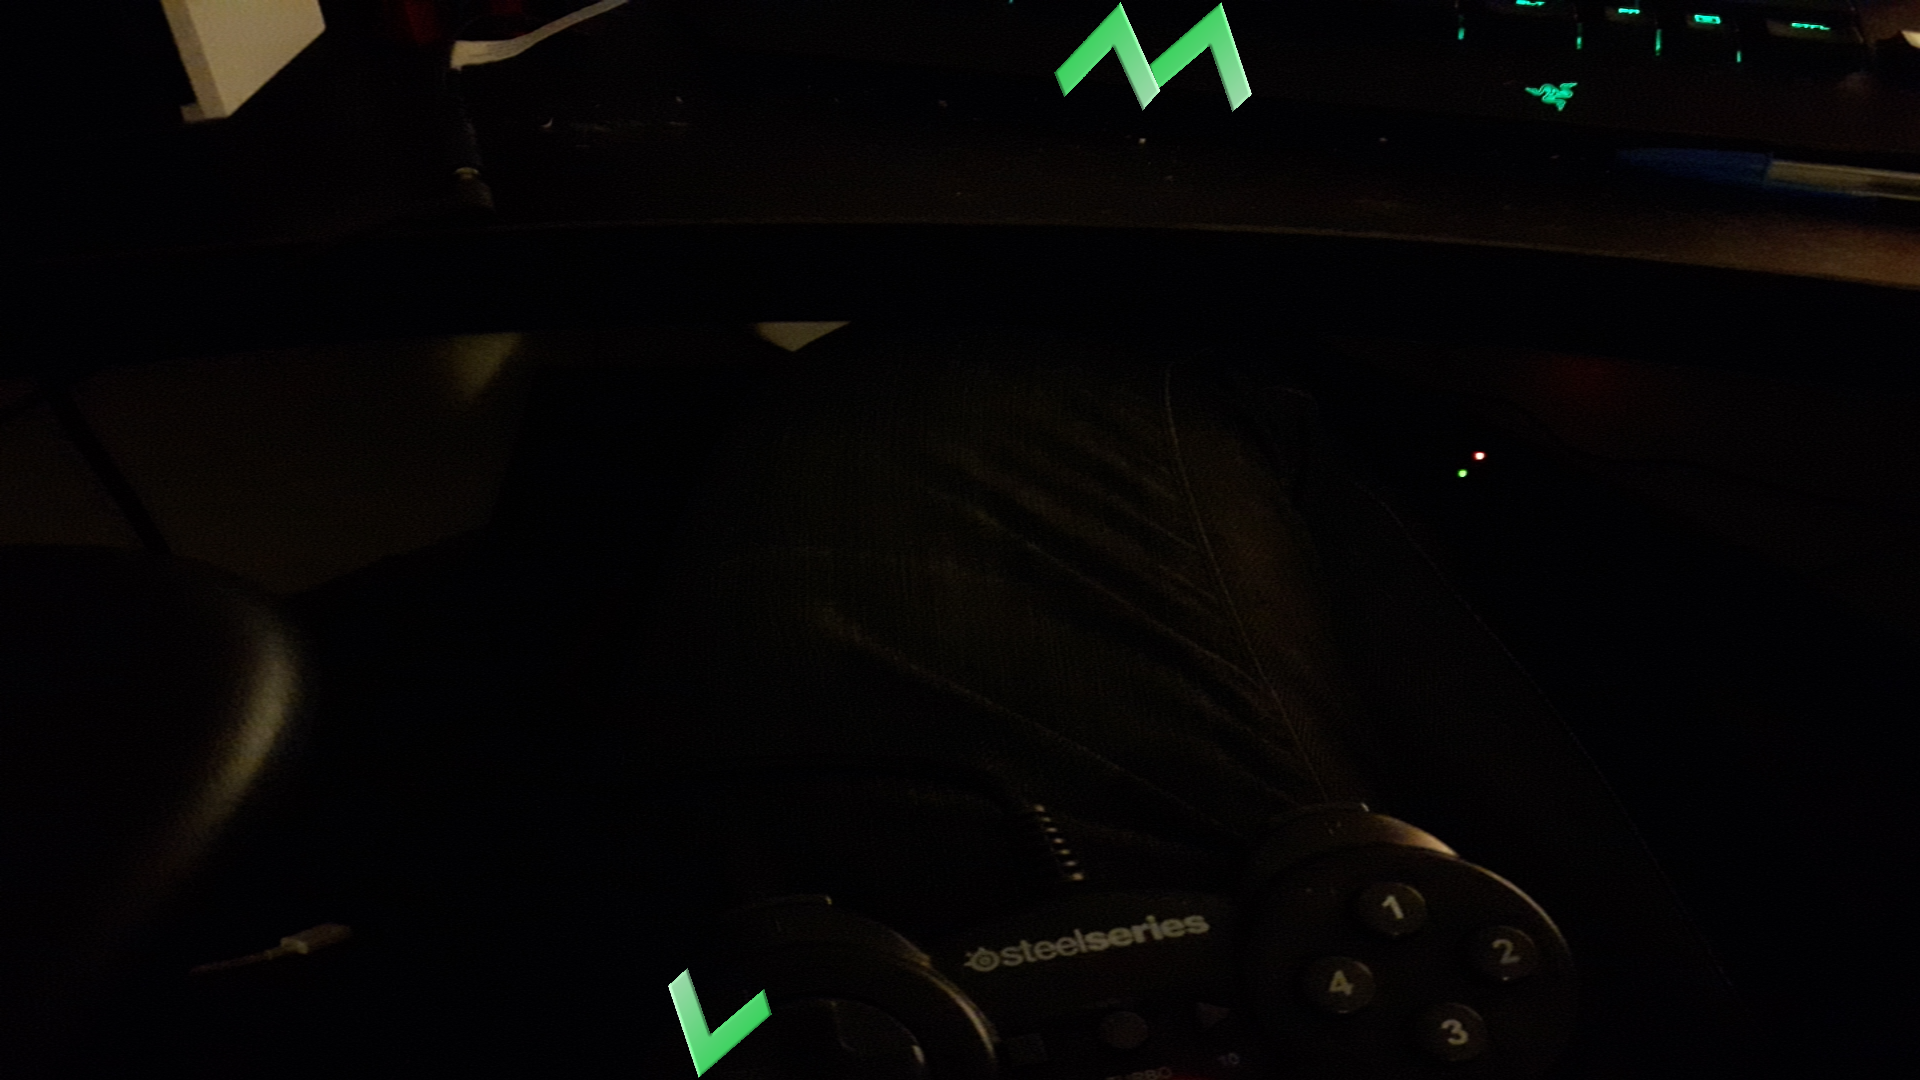
\includegraphics[width=8cm]{Figures/OffscreenPositions2.png}
	\decoRule
	\caption{Offscreen tag positions are shown with a green arrow}
	\label{fig:Billboarding}
\end{figure}

One of the advantages of AR is the ability to put more information on the screen than can be seen with the human eye. As part of the goal of the project to increase the user's awareness of the locations of objects, the system informs the user of where an object is relative to them when the object is not within the viewing area of the camera.

First, the system needs to determine whether or not the objection is within the viewing area. This is done by multiplying the object's position in space relative to the camera by the view and projection matrices. That is, given a position $p$, we find the NDCs of $p$, $p_{NDC}$, by:

\[ p_{NDC} = \mathbf{P} \mathbf{V} p \]

If the point is outside the bounding box from $(-1, -1, -1)$ to $(1, 1, 1)$, then the point is known to not be visible on the screen. Or, since $p_{NDC}$ is in homogenous coordinates, we can check whether any of the components are greater than or less than $w$.

In code:

\begin{lstlisting}[language=Java]
//Start by determining whether or not this is on the screen
float[] p = {x, y, z, 1}; //w=1 by default
float[] pNDC = new float[4];
 Matrix.multiplyMV(pNDC, 0, vpMatrix, 0, p, 0);

boolean onScreen = true;
for (int i = 0; i < 3; i++) {
	//if v outside the bounds -w <= x_i <= w
	if (pNDC[i] <= -pNDC[3] || pNDC[i] >= pNDC[3]) {
		onScreen = false; //is clipped
	}
}

//onScreen is now false if the point is off the screen
\end{lstlisting}

The system displays an arrow on the edge of the screen pointing towards where the object is. To determine the angle and the part of the screen where the arrow should be drawn, we continue to use $p_NDC$.

The direction of the arrow can be determine by the vector from the center of the screen, $(0, 0, 0)$ in NDCs, to $p_{NDC}$. The z component is ignored (as we are rendering a 2D arrow not a 3D arrow there is no way to add a tilt using the z contribution), and we only look at the xy components of the point. Then, the edge of the screen where the arrow should go is given in NDCs as where that vector intersects the bounding box from $(-1, -1)$ to $(1, 1)$. This intersection is calculated by dividing $p_{NDC}$ by the larger of its components, so that the magnitude of the larger component is 1 and the magnitude of the smaller component is some number smaller than 1. The new point is $p_{edge}$.

The point is transformed back into world coordinates by multiplying the inverse of the view-projection matrix by it. Then, the square textured with an arrow image on it is rotated an amount determined by where the point is on the screen so it will point in the same direction as the vector from the NDCs $(0, 0, 0)$ to $p_{NDC}$. 

In code:

\begin{lstlisting}[language=Java]
float divisor = Math.max(Math.abs(x), Math.abs(y));
//homogenous component set to 1, z value determines how large the arrow is later
float[] edgeVector = {x/divisor, y/divisor, 0.6f, 1}; 

//Rotate based on vector in NDC, then rotate on inverted view matrix so it faces the camera
float[] rotateToFaceEdgeMatrix = new float[16];
Matrix.setIdentityM(rotateToFaceEdgeMatrix, 0);
float angle = (float)Math.atan2(edgeVector[1], edgeVector[0]);
Matrix.rotateM(rotateToFaceEdgeMatrix, 0, angle*180f/(float)Math.PI, 0, 0, 1f);
//correct so the right edge is on the right border
Matrix.translateM(rotateToFaceEdgeMatrix, 0, -0.5f, 0, 0); 

//Face camera...
float[] rotationMatrix = new float[16];
Matrix.multiplyMM(rotationMatrix, 0, invertedViewMatrix, 0, rotateToFaceEdgeMatrix, 0);

//Convert from NDC to world coordinates via inverted VP matrix, translate matrix to that
float[] worldCoords = new float[4];
Matrix.multiplyMV(worldCoords, 0, invertedVPMatrix, 0, edgeVector, 0);
Math3D.fixHomogenous(worldCoords); //w may be non-1

float[] translationMatrix = new float[16];
Matrix.setIdentityM(translationMatrix, 0);
Matrix.translateM(translationMatrix, 0, worldCoords[0], worldCoords[1], worldCoords[2]);

float[] modelMatrix = new float[16];
Matrix.multiplyMM(modelMatrix, 0, translationMatrix, 0, rotationMatrix, 0);

return modelMatrix;
\end{lstlisting}

An example of the rendered off-screen arrow can be seen in (TODO).

\section{Results}
Show off how accurate we are. Have Youtube videos displaying such.

\section{Summary}
This chapter dealt with a number of topics related to rendering the position markers this project requires.

First, the chapter dealt with a brief overview of transformation matrices and homogenous coordinates. Transformation matrices are used to scale, rotate, and translate vertices. Homogenous coordinates are regular coordinates with an added $w$ component which acts to scale the rest of the components in the vector.

OpenGL renders a 3D scene using three main matrices: the model matrix, which converts from a model to the world, the view matrix, which then transforms the vertices so they face the camera, and finally the projection matrix, which converts from view space to coordinates of the cellphone's screen.

Objects can be made to face the screen via billboarding. In this project, 3D squares are used which are textured with the marker and arrow images. To make the squares face the camera, the 3D objects are rotated on all three axes by multiplying by the inverse of the rotational part of the view matrix.

Android's API for getting the rotation of the cellphone was discussed. The rotation matrix is very accurate, but becomes inaccurate when the device is in motion. A calibration rotation matrix is constructed to transform the position calculation subsystem's positions into coordinates that can be mapped to the real world.

The accuracy of the AR subsystem is discussed. TODO
